\chapter{Especificación del Problema}

% Descripción detallada del problema a resolver
% Se discute la relevancia de contar con una solución
% Se especifica en todo detalle los requisitos de la solución a construir
% Características de calidad de la solución deseada
% Es deseable también establecer criterios de aceptación de una solución al problema

\section{Descripción del problema}

\todo[inline]{Explicar que las líneas ya han sido detectadas. Como? Mencionar o citar el trabajo de Karim Pichara y Andrés Riveros?}

Supóngase que se cuenta con conjuntos de espectros, y que cada uno de ellos posee todas sus líneas espectrales correctamente detectadas y, por lo tanto, se conoce su posición en el espectro. En la práctica eso puede ser muy difícil de lograr, sobre todo en circunstancias donde pueden existir en principio una alta cantidad de líneas espectrales y estas pueden interferir unas con otras en la señal final, lo que se conoce como \textit{blending}.\todo[inline]{No sé si poner lo anterior acá o en el capítulo de marco teórico} Por lo tanto, para efectos de lo que sigue, basta con asumir que existe la posibilidad que no todas las líneas hayan sido detectadas. Pero es importante que las que sí fueron detectadas, lo hayan sido con una seguridad suficiente y que se sepa de manera adecuada su posición.\todo[inline]{Explicar cómo se llevó a cabo la detección en términos más rigurosos. Cómo?}

Teniendo estos conjuntos de espectros con sus respectivas líneas detectadas se desea... 

\todo[inline]{Definir el problema de forma general, quizás con lineamientos de objetivos, que no involucre directamente como solución el uso de reglas de asociación}

\section{Requisitos de la solución y casos de uso}

A continuación se enuncian los requerimientos del sistema:

\begin{enumerate}
	\item \textbf{Obtener reglas de asociación entre líneas de emisión espectrales [esencial].} \\
	El sistema debe generar reglas de asosiación entre líneas de emisión presentes en espectros de frecuencia, independientemente de si estos pertenecen a una misma o a distintas moléculas o átomos, o si no han sido aun identificadas.
	\item \textbf{Permitir al usuario observar las reglas generadas, y las medidas de relevancia de cada una de ellas, y guardar estos resultados [esencial].} \\
	Una vez extraídas las reglas de asociación, el usuario debe poder revisarlas y guardarlas para su revisión posterior.
	\item \textbf{Permitir al usuario aplicar los mismos algoritmos de reglas de asociación a datos de diversas fuentes [esencial].} \\
	Se desea que el sistema de extracción sea lo más general posible, de modo tal de poder aplicarlo a datos de líneas espectrales extraídos de distintos \textit{surveys}, bases de datos, sistemas de modelamiento y detección de líneas, entre otros.
	\item \textbf{El sistema debe ser ejecutable en un ambiente de computación de alto rendimiento [deseable].}
	\item \textbf{El sistema debe ser compatible con plataformas de observatorios virtuales [deseable].} 
	\item \textbf{Implementar una interfaz gráfica de usuario [opcional].}
\end{enumerate}

\subsection{Casos de Uso}

En la Figura \ref{fig:cases} se muestra un diagrama con los casos de uso preliminares del sistema a desarrollar.

\begin{figure}[h!]
\begin{center}
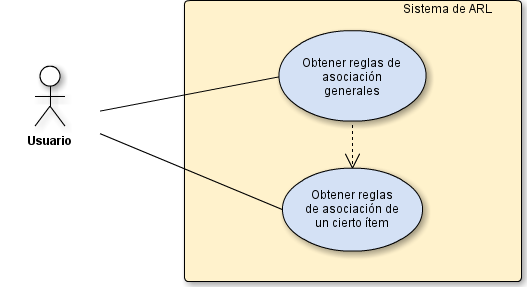
\includegraphics[width=14cm]{imagenes/casos_de_uso.png}
\end{center}
\vspace*{-5mm}
\caption{Diagrama de casos de uso del sistema.}
\label{fig:cases}
\end{figure}

\subsubsection{Actores}

Para este sistema existe solo un tipo de actor, dado que todos los usuarios finales tendrán acceso a las mismas funcionalidades. Este usuario será el encargado de seleccionar el conjunto de datos que quiere ingresar al sistema, en forma de vectores de líneas moleculares. Cada vector poseerá las líneas identificadas en un espectro de frecuencia en particular. Este usuario ingresará estos datos al sistema y luego seleccionará los parámetros de detección de reglas que desee. Una vez ejecutados los algoritmos correspondientes, el usuario podrá observar las reglas generadas y, si así lo desea, ajustar nuevamente los parámetros para obtener mejores resultados sobre el mismo conjunto de datos.

Posteriormente, el mismo u otro usuario podrá verificar los resultados obtenidos en una sesión de ARL anterior y ajustar los parámetros de búsqueda a su agrado para luego volver a correr los algoritmos sobre los mismos iniciales.

\subsubsection{Descripción de casos de uso}

En la siguiente tabla se muestra una descripción detallada de los casos de uso y se indica, de ser así, a qué requerimiento está asociado.

\begin{tabular}{|l|p{4cm}|p{7cm}|l|l|}
	\hline
	ID & Caso de uso & Descripción & Tipo & Ref. \\ \hline
	1 & Ejecutar ARL sobre datos con rangos espectrales idénticos & El usuario selecciona un conjunto de espectros extraídos a partir de un sólo cubo de datos o de más de uno, pero siempre en rangos de frecuencia idénticos, selecciona los parámetros adecuados y ejecuta los algoritmos de ARL sobre ellos. & Esencial & 1,2,4 \\ \hline
	2 & Ejecutar ARL sobre datos con distintos rangos espectrales & El usuario selecciona un conjunto de espectros extraídos a partir de dos o más cubos de datos con distintos rangos de frecuencia, selecciona los parámetros adecuados y ejecuta los algoritmos de ARL sobre ellos. & Esencial & 1,2,3 \\ \hline
	3 & Verificar resultados & El usuario examina las reglas generadas por los algoritmos determinando si le dan información valiosa o si, en su defecto, necesita volver a ejecutarlos con distintos parámetros & Esencial & 3 \\ \hline
\end{tabular}
